%% TODO fix the case study so that the time complexity is not as high
%% TODO say what operator will be used, why it's good and what the alternatives are
%% TODO say what the issues with rank-based selection are and why it's a good fit here
%% TODO say what the issues with cross-over are and why / why not it's a good fit here
%% TODO is the phenotype the timetable OR a list of lectures?

%% options: [no]titlepage, twocolumn, landscape, draft
\documentclass[a4paper, 12pt, titlepage]{article}
\usepackage{graphicx}
\usepackage{titlesec}

\titlespacing*{\section}
{0pt}{1.0ex plus 1ex minus .2ex}{1.0ex plus .2ex}
\titlespacing*{\subsection}
{0pt}{1.0ex plus 1ex minus .2ex}{1.0ex plus .2ex}
\usepackage[utf8]{inputenc}
\usepackage[english]{babel}
\usepackage[margin=0.1in]{geometry}

\usepackage{minted}
\date{} % overwrite default format
\author{Norbert Logiewa\\nl253}
\title{Applications of Evolutionary Algorithms in \\Scheduling, Planning and Timetabling}

\begin{document}

\maketitle

Evolutionary algorithms (EA) are a class of procedures that are
used when finding a solution to a problem using regular means is not
possible or very difficult. EAs are often employed when dealing with
multi-dimensional problems where sampling of every candidate is not
possible \cite[p.~29]{floreano2008}. This essay will discuss how GA can
be applied to scheduling.  \emph{Scheduling} and \emph{timetabling}
in this essay will refer to ordering of tasks that aims to maximise
the productivity.  The ordering may schedule some activities to take
place in parallel if business rules and the amount of resources allow
for that.  Efficient scheduling of tasks if of interests to anyone who
wishes to increase their productivity \emph{without} investing additional
resources.  EAs allow to find good-enough solution to problems that don't
necessarily need an \emph{optimal} solution\cite[p.~44]{heaton2014}.
This is often because the search space is too large to be directly
traversed so brute-force methods are not possible.

% \emph{Productivity} will refer the extent to which a schedule helps some
% organisation to achieve their goals. \footnote{If, for example, we are
% scheduling for a web development agency, we can measure productivity by
% the lines of code produced by the developers.}

\section*{Case Study -- University}

A hypothetical university may wish to improve the productivity of students
and lecturers by using an EA for timetabling. Suppose the university
offers 200 modules to 16000 students. Each year every student must take 8
unique modules. Each module needs to have 2 one-hour lectures during the
working week. Additionally, each of those lectures or can take place in
one of 50 lecture halls. Moreover, each of those lectures may be given
by a lecturer from the relevant department.  Finally, each lecture or
may take place a time between 9am and 7pm.  The task would be to ensure
that: every student and lecturer is in at most one lecture at a time,
only one lecture takes place in a lecture hall at the same time, etc.
A timetable i.e. a candidate solution that obeys all of these business
rules would be favoured in the process of natural selection and would
receive a higher fitness score as evaluated by the fitness function.

% As input the GA would take a set of combinations of modules that the students chose.

\section*{Solving the Problem}

GA is well suited for the task because there is likely many good-enough
solutions to the problem i.e. many timetables could satisfy the
constraints listed above. In other words, the fitness landscape has
many peaks, hence, using a global-search algorithm is beneficial.
Furthermore, the complexity of the problem (large search
space and multiple dimensions) means that a brute force search in this
multi-dimensional space would take too much time.

\subsection*{Phenotype and Genotype}

Each candidate solution (timetable) would be encoded as a bit-string
\footnote{this is the genotype and is analogous to DNA} representing all
the lectures along with time, place and the lecturer taking place during
the week.  This choice of bitstring encoding for candidate representation
is motivated by the fact that this encoding has been extensively discussed
in the literature on GA \cite[p.~103]{eberhart2007}. Bitstrings are
the most common encoding \cite[p.~127]{norvig2010} possibly because
this low-level representation uses less resources and operators such as
cross-over mutation invented by researchers tend to behave well when we
encode solutions in this manner.  The crossover operator, for instance,
is extremely easy to apply to a bit-string but less easy to other
data structures such as sets.  In this scenario we allocate a chunk
of bits for every lecture that must take place.  In every sub-string
representing a lecture the first bit determines whether the lecture
takes place in the first or the second semester.  The following \(m\)
bits encode an integer index in the modules array.  The next \(l\)
bits encode an integer index in a lecturer array. The following \(t\)
bits encode an integer referring to the time that lecture will take
place. The last \(h\) bits encode an integer index in a lecture halls
array. Hence each lecture is be a bit-string of length \(1 + m + l + t +
h\) and each candidate is be a concatenation of \(400\) of these giving
us in total a bit-string of length \(400(1 + m + l + t + h)\). If we
delegate, say, 16 bits to representing the time and 8 for each indexing
integer, we end up with each candidate having a size of \(400 * (1 +
8 + 8 + 8 + 16)\ bits = 16400\ bits = 2050\ Bytes = approx.\ 2\ KB \).
It's useful to bear in mind the size of each candidate when deciding on
the population size. Some researchers suggest population sizes of \(1000\)
\cite[p.~25]{heaton2014}. This would mean our application would require
\(2\ KB * 1000 = 2000\ KB = 2\ MB\) memory.  The \emph{phenotype} might be a
list of lectures, for instance, which we would decode from the \emph{genotype}
(bitstring).

\subsection*{Selection Operator}

The GA literature discusses a number of operators to be used for
selection: proportionate, rank-based and tournament among others
\cite{floreano2008, eberhart2007, heaton2014}.  A good choice of selection
operator would be rank-based selection (RBS). The reason for this is that
in this scenario the exact fitness value of an individual is irrelevant.
It's sufficient to know that a candidate is better than others for it
to make it into the next gene-pool.  Moreover, It's not clear that other
more sophisticated selection methods such as tournament selection would
yield better results. Furthermore, RBS avoids issues that proportionate
selection faces: when all candidates have a similar fitness or one
candidate has a large high fitness score, the selection turns into a
random search.  \cite[p.~23]{floreano2008} Lastly, the use of RBS simplifies
implementation and is in line with the principle of parsimony.

\subsection*{Genetic Operators \& Adaptive GA}

Application of a selection operator reduces the size of the population. To
replenish it, pairs of winners are used as input to the crossover operator which creates
new individuals.  Crossover is used because it is a standard and
well-understood operator. Additionally, mutation is introduced with
a small probability to further increase variation in the population.
These two tend to be combined because cross-over \emph{recombines} existing
genes whereas mutation introduces \emph{novelty}.  \cite[p.~27]{heaton2014}.
A good starting values for the parameters would be as follows:
\(p(crossover) = 0.8\) \cite[p.~117]{eberhart2007} and \(p(mutation) =
0.2\) \cite[p.~25]{heaton2014} although some researchers suggest lower
rates e.g. \(0.005\) \cite[p.~117]{eberhart2007}.

However, the crossover operator is problematic. In the initial phase
of looking for a solution across the fitness landscape it is useful to
vary candidates a lot so using crossover is highly beneficial. However,
once a satisfactory candidate has been found, we might only wish to
tweak it a bit. Altering the candidate too much would be equivalent
to abandoning the progress that has been made to reach this fitness
score. Hence, a less "invasive" and more fine-grained operator such
as mutation \cite[p.~28]{floreano2008} may become more advantageous as
the number of iterations grows.  In a bit-string a mutation would flip
a bit which may, for example, increment an integer which represents
a lecturer thus making a change in a candidate.  The benefit of using
crossover, arguably, diminishes with time. To implement that we might
increase the probability of mutation and increase the probability of cross-over 
at the beginning of every iteration until \(p\) reaches \(0\) for cross-over
and until \(p\) reaches \(1\) for mutation.

An alternative way of preserving the fittest candidates in the next
population would be to use elitism. This would protect against degrading
of solutions when cross-over is applied to fittest candidates.
\cite[p.~26]{floreano2008}

However, this enhancement may not be necessary. Norvig
\cite[p.~128]{norvig2010} points out that when the algorithm begins to
converge on a solution after being run for a while, the candidates in
our population are not very diverse. This means, in theory, that the
cross-over operator would take "smaller steps" because of how similar
candidates are.

\subsection*{The fitness function}

The fitness function deciphers each of the \(400\) sub-strings within each
candidate bit-string and assigns a score to each candidate which reflects
the extent to which it obeys the business rules. \cite[p.~22]{floreano2008} 
In pseudo (python-like) code: 

\inputminted{python}{fitness.py}

The pseudocode illustrates that the fitness function has a bad \(O(l^2 *
c)\) complexity where: \(l\) = number of lectures \footnote{in this
scenario \(l = 200 * 2\)} for all modules and \( c = \) number of
combinations of modules.  Initially it may seem that the fitness function
is not computationally feasible.  With 200 modules and 8 modules to be
takes for every student the maximum number of combinations is \(8C200 =
55098996177225\). However, there are bound to be restrictions on the
combinations of modules. For example, a computer science student is
unlikely to be allowed to take "Introduction to Criminology". In fact, we
would expect each student to only be able to choose from around 15 modules
from their own department. \(8C15 = 6435\) is a much more manageable number.
\footnote{the pseudo-code assumes that module configurations for all students are presented
in a multiset where every key is itself a set of modules (similar to frozen sets in
Python, see https://docs.python.org/3/library/stdtypes.html#frozenset)
and value is the number of students who chose this particular combination of modules}

\subsection*{The invariant}

GA is run repeated until either enough time has passed or other condition
has been met. \cite[p.~108]{eberhart2007}. In this scenario a good choice
would be to wait for a high enough fitness value in a candidate but to
also introduce a timeout of, say, 10 minutes in case such a candidate
cannot be found.

\section*{Summary}

The basic idea behind this particular version of GA is described by the
following UML activity diagram: 

\begin{figure}[h]
    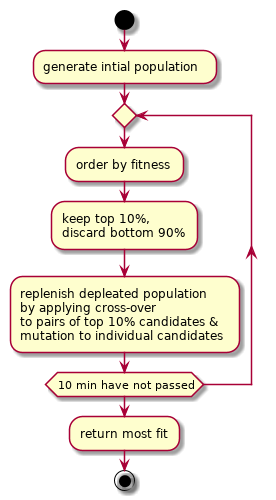
\includegraphics[scale=0.6]{algo.png}
    \centering
\end{figure}

This essay demonstrated how EA can be used to aid timetabling and
scheduling. It illustrated how to apply EA using a case study of a
university, it discussed how to encode the candidate timetables and
stated how carry out the algorithm in this scenario.

\begin{thebibliography}{9}

  %% 1 authors
  %% 2 title of the paper
  %% 3 name of conference/journal/book where it was published
  %% 4 number of the volume and issue in the case of journals
  %% 5 page numbers of the paper
  %% 6 publisher
  %% 7 year or month and year for journals
  
  \bibitem{norvig2010}
  Stuart Russel and Peter Norvig,
  \textit{Artificial Intelligence},
  \textit{A MODERN APPROACH},
  p. 126-129, 
  3rd Ed., 
  Pearson Education
  2010.

  \bibitem{floreano2008}
  Dario Floreano and Claudio Mattiussi,
  \textit{Bio-Inspired Artificial Intelligence},
  \textit{THEORIES, METHODS, AND TECHNOLOGIES},
  p. 1-38,
  MIT Press,
  2008.

  \bibitem{eberhart2007}
  Russel C. Eberhart,
  \textit{Computational Intelligence},
  \textit{Concepts to Implementations},
  p. 103-118,
  p. 51-68,
  Denise E.M. Penrose,
  2007.

  \bibitem{heaton2014}
  Jeff Heaton,
  \textit{Artificial Intelligence for Humans},
  \textit{Volume 2: Nature Inspired Algorithms},
  p. 1-100,
  Heaton Research, Inc,
  2014.

\end{thebibliography}

\end{document}
